\batchmode
\documentclass[
%8pt, 9pt, 10pt, 11pt, 12pt, 14pt, 17pt, 20pt
%serif,
%table, % for table coloring
%draft,
%ngerman,
%handout,	% remove overlays
compress,
xcolor=table,
dvipsnames,
]{beamer}

\usepackage{tipa}
%% Encoding, fonts, language
%% Font & Encoding
%\usepackage{libertine}
\usepackage[libertine]{newtxmath}
\usepackage[scaled=0.8]{beramono}  % for monospaced font
\usepackage{microtype}		% micro-typographic aspects of the fonts
\usepackage[T1]{fontenc}	% special fonts, e.g. for German umlaute
%% incompabtible with Biblatex
% \usepackage{ucs}
% \usepackage[utf8x]{inputenc}
%% compatible with Biblatex
\usepackage[utf8]{inputenc}



%% Language
\usepackage[spanish]{babel}


 


\usepackage{etex} 
\usepackage{graphics}
\usepackage{subcaption}
%%%%%%%%%%%%%%%%%%%%%%
%   TIKZ SETTINGS    % 
%%%%%%%%%%%%%%%%%%%%%%

\usepackage{tikz}
%%%%%%%%%%%%%%%%%%%%%%%%%%%%%%%%%%%%%
% tikz-qtree bugfix by Andrew Stacey  
\makeatletter
 
\def\unwind@subpic#1{%
% is #1 the current picture?
\edef\subpicid{#1}%
\ifx\subpicid\pgfpictureid
% yes, we're done
\else
% does #1 have a parent picture?
\expandafter\ifx\csname pgf@sh@pi@#1\endcsname\relax
% no, the original node was not inside the current picture
\pgf@xa=\pgf@x
\pgf@ya=\pgf@y
\pgfsys@getposition{\pgfpictureid}\pgf@shape@current@pos
\pgf@process{\pgfpointorigin\pgf@shape@current@pos}%
\advance\pgf@xa by-\pgf@x%
\advance\pgf@ya by-\pgf@y%
\pgf@process{\pgfpointorigin\subpic@parent@pos}%
\advance\pgf@xa by \pgf@x%
\advance\pgf@ya by \pgf@y%
\pgf@x=\pgf@xa
\pgf@y=\pgf@ya
\else
% yes, apply transform, save picture location, and move up to parent picture
\pgfsys@getposition{\csname pgf@sh@pi@#1\endcsname}\subpic@parent@pos%
{%
  \pgfsettransform{\csname pgf@sh@nt@#1\endcsname}%
  \pgf@pos@transform{\pgf@x}{\pgf@y}%
  \global\pgf@x=\pgf@x
  \global\pgf@y=\pgf@y
}%
\unwind@subpic{\csname pgf@sh@pi@#1\endcsname}%
\fi
\fi
}


\def\pgf@shape@interpictureshift#1{%
\def\subpic@parent@pos{\pgfpointorigin}%
\unwind@subpic{\csname pgf@sh@pi@#1\endcsname}%
}

\makeatother
% tikz-qtree bugfix by Andrew Stacey 
%%%%%%%%%%%%%%%%%%%%%%%%%%%%%%%%%%%%%

\tikzset{every tree node/.style={align=center,anchor=north}}	% to allow linebreaks
\usetikzlibrary{calc} % for positioning arrows with ($(t.center)-(1,0)$)
\usetikzlibrary{shapes,decorations}
\usetikzlibrary{backgrounds,fit}
\usetikzlibrary{arrows}
\usetikzlibrary{matrix}
\usetikzlibrary{positioning}
\usetikzlibrary{automata}
\usetikzlibrary{tikzmark}

% Define box and box title style (see http://www.texample.net/tikz/examples/boxes-with-text-and-math/)
\tikzstyle{mybox} = [draw=gray, very thick,
    rectangle, rounded corners, inner sep=10pt, inner ysep=17pt,yshift=3pt]
\tikzstyle{fancytitle} =[draw=gray, very thick, fill=white,
    rectangle, rounded corners, inner sep=5pt, inner ysep=5pt]
\tikzstyle{mydouble} = [double distance=1pt]
    
\tikzset{
    %Define standard arrow tip
    >=stealth',
    %Define style for boxes
    box/.style={
           rectangle,
           rounded corners,
           draw=black, very thick,
           text width=10em,
           minimum height=2em,
           text centered},
    % Define arrow style
    arrow/.style={
           ->,
           thick,
           	shorten <=2pt,
           shorten >=2pt,}
}

\newcommand\centertikz[1]{\tikz[baseline=(current bounding box.center)]{#1}}
\newcommand\tikzcenter{baseline=(current bounding box.center)}
\newcommand\tikztop{baseline=(current bounding box.north)}

\newcommand\tikztreeset[1]{\matrix [matrix of nodes,left delimiter=\{,right delimiter=\}](set){#1};} 
\usepackage{forest}

\makeatletter

\@ifpackagelater{forest}{2016/01/01}
{\useforestlibrary{linguistics}}
{}

\@ifpackagelater{forest}{2016/01/01}
{\newcommand{\forestPreamble}{default preamble}} % version >=2 of forest
  {\newcommand{\forestPreamble}{.style}} % version <=1 of forest

\makeatother
  
\forestset{
  \forestPreamble ={
	% % .style={ % version <=1 of forest
	% default preamble={ % version >=2 of forest    
		for tree={
			parent anchor=south, 
			child anchor=north,
			% align=center,			% bad: adds space below label
			fit=rectangle,
			base=top,				% vertical orientation of nodes
			% inner sep=3,			% necesssary?
			begin draw/.code={\begin{tikzpicture}[baseline=(current bounding box.center)]},
			}},
    sn edges/.style={for tree={parent anchor=south, child anchor=north}},
    red subtree/.style={for tree={text=red},for descendants={edge=red}},
    black subtree/.style={for tree={text=black},for descendants={edge=black}},
    gray subtree/.style={for tree={text=gray},for descendants={edge=gray}},
    vcenter/.style={begin draw/.code={\begin{tikzpicture}[baseline=(current bounding box.center)]}},
      empty nodes/.style={	% from the forest manual
        for tree={
          % calign=fixed edge angles,
          yshift=1ex},
        delay={where content={}{shape=coordinate,for parent={for children={anchor=north}}}{}}},
      derivation tree/.style={.style={
          for tree={parent anchor={},child anchor={},font=\ttfamily}}},
      dt label/.style 2 args={
        edge label={node[midway,font=\ttfamily\scriptsize, #1]{#2}},},
    }

   

    

\usepackage{url}
\usepackage{amsmath,amssymb,amsfonts,marvosym}
\usepackage{ulem}			% to cross out text
\normalem

\usepackage{ragged2e}
\let\raggedright=\RaggedRight

%\usepackage[utf8]{inputenc} %Este es el paquete para que te muestre bien los caracteres latinos
%\usepackage[useregional]{datetime2} %paquete para la fecha

\usepackage{linguex}   % must be loaded below \usepackage[T1]{fontenc}
\AtBeginDocument{
  \setlength{\Exlabelsep}{0em}		% for linguex examples
  \setlength{\SubExleftmargin}{1,5em}	% for linguex examples
  \renewcommand\eachwordone{\sffamily}	% for glossing with linguex
  \renewcommand\eachwordtwo{\sffamily}	% for glossing with linguex
  % \setlength{\Extopsep}{1ex}   % vertical margin in linguex examples
}
%%%%%%%%%%%%%%%%%%%%%%
%   AVM SETTINGS     % 
%%%%%%%%%%%%%%%%%%%%%%

\usepackage{packages/avm}

\avmoptions{center} 
\avmfont{\scshape}
\avmvalfont{\normalfont}
\avmsortfont{\normalfont\itshape}

\newenvironment{topbot}{   	% more flexible than /newcommand ?
	\avmvskip{0.2ex} 
	\hspace{-1.5em}
	\begin{avm}
	\avml
	}
	%%%
	{
	\avmr
    \end{avm}
    \hspace{-0.5em}
}

%%%%%%%%%%%%%%%%%%%%%%%%
%   BEAMER SETTINGS    % 
%%%%%%%%%%%%%%%%%%%%%%%%

%\usefonttheme{serif}
%\renewcommand*{\ttdefault}{cmtt}

\definecolor{HHUblue}{HTML}{006AB3}
\setbeamercolor{structure}{fg=HHUblue}

\setbeamerfont{frametitle}{family=\sffamily}
\setbeamerfont{title}{family=\sffamily}
\setbeamerfont{block title}{family=\sffamily}

\usetheme{Copenhagen} % Boadilla
\usecolortheme{default}   % beaver
\usefonttheme{default}		% default | professionalfonts | serif | structurebold | structureitalicserif | structuresmallcapsserif
\useinnertheme{default} 	% circles | default | inmargin | rectangles | rounded
\useoutertheme{default}	% default | infolines | miniframes | shadow | sidebar | smoothbars | smoothtree | split | tree

%\setbeamercovered{transparent}				% for transparent overlays
\setbeamercovered{invisible}				% for non-transparent overlays
\setbeamertemplate{navigation symbols}{}	% no navigation symbols
\setbeamertemplate{headline}[default]		% no headline
\setbeamertemplate{footline}[frame number]
\setbeamertemplate{section in toc}[]
\setbeamertemplate{subsection in toc}[]
\setbeamertemplate{itemize items}[square]
\setbeamertemplate{enumerate items}[square]
%\setbeamertemplate{blocks}[default]		% rectangular blocks
%\setbeamersize{text margin left=10pt,text margin right=10pt}

%% Bibliography style (http://tex.stackexchange.com/questions/97615/article-style-bibliography-in-beamer-class)
\setbeamertemplate{frametitle continuation}[from second]
% Now get rid of all the colours
\setbeamercolor*{bibliography entry title}{fg=black}
\setbeamercolor*{bibliography entry author}{fg=black}
\setbeamercolor*{bibliography entry location}{fg=black}
\setbeamercolor*{bibliography entry note}{fg=black}
% and kill the abominable icon
\setbeamertemplate{bibliography item}{\insertbiblabel}  % insert label from bib(la)tex
\AtBeginDocument{
  \renewcommand*{\bibfont}{\scriptsize}
}

\tikzset{% makes available \only and \alt inside paths
  only/.code args={<#1>#2}{\only<#1>{\pgfkeysalso{#2}}},
  alt/.code args={<#1>#2#3}{\alt<#1>{\pgfkeysalso{#2}}{\pgfkeysalso{#3}}}
}

\setbeamertemplate{footline}
{
  \leavevmode%
  \hbox{%
    \pgfsetfillopacity{0}\begin{beamercolorbox}[wd=.333333\paperwidth,ht=2.25ex,dp=1ex,left]{author in head/foot}%
      \usebeamerfont{author in head/foot}\pgfsetfillopacity{1}\color{gray}\hspace*{2ex}\insertshortauthor~~(\insertshortinstitute)
    \end{beamercolorbox}%
    \pgfsetfillopacity{0}\begin{beamercolorbox}[wd=.333333\paperwidth,ht=2.25ex,dp=1ex,center]{title in head/foot}%
      %\usebeamerfont{title in head/foot}\pgfsetfillopacity{1}\insertshorttitle
    \end{beamercolorbox}%
    \pgfsetfillopacity{0}\begin{beamercolorbox}[wd=.333333\paperwidth,ht=2.25ex,dp=1ex,right]{date in head/foot}%
      \usebeamerfont{date in head/foot}\pgfsetfillopacity{1}\insertshortdate{}\color{gray}\hspace*{2em}
      \insertframenumber{} %/ \inserttotalframenumber
      \hspace*{2ex}
    \end{beamercolorbox}}%
  \vskip0pt%
}


\newcommand{\separationframe}[1]{
\begin{frame}
\frametitle{}

\begin{center}
  \LARGE 
  \settowidth{\stmueTmp}{ #1 }
    \begin{minipage}{\stmueTmp}
    \begin{block}{}
    \begin{center}
    %\usebeamercolor[fg]{frametitle}
    #1
    \end{center}
    \end{block}
    \end{minipage}
\end{center}

\end{frame}
}

\newcommand\framecite[1]{
\vskip-2ex
\hfill #1%
\vskip-3.3ex ~
}

%% Bibliography
%% BibLaTeX
\newcommand{\mycitestyle}{bst/sp-authoryear-comp}
\makeatletter
\@ifclassloaded{beamer}{\renewcommand{\mycitestyle}{numeric-comp}}{}
\makeatother

\usepackage[
  natbib=true,
  style=bst/biblatex-sp-unified,
  citestyle=\mycitestyle,
  %refsection=chapter,
  maxbibnames=99,
  isbn=false,
  doi=false,
  eprint=false,
  %backend=biber,
  backend=bibtex,
  % sorting=ydnt,  % sort in descending chronological order
  indexing=cite,
  labelnumber,  % for numeric bibliography in beamer
  %toc=bib    % make bibliography appear in toc, incompatible with beamer
  ]{biblatex}
\renewcommand{\postnotedelim}{: }%
\renewcommand{\multicitedelim}{\addsemicolon\space}%
\renewcommand{\compcitedelim}{\multicitedelim}%
\DeclareFieldFormat{postnote}{#1}%

%% beamer settings
\makeatletter
\@ifclassloaded{beamer}{  
  \DeclareFieldFormat{labelnumberwidth}{[#1]}
  \defbibenvironment{bibliography}  % from numeric.bbx
      {\list
        {\printtext[labelnumberwidth]{%
          \printfield{prefixnumber}%
          \printfield{labelnumber}}}
        {\setlength{\labelwidth}{\labelnumberwidth}%
            \setlength{\leftmargin}{\labelwidth}%
            \setlength{\labelsep}{1em}%
            \addtolength{\leftmargin}{1em}%
            \setlength{\itemsep}{\bibitemsep}%
            \setlength{\parsep}{\bibparsep}}%
            \renewcommand*{\makelabel}[1]{\hss##1}}
      {\endlist}
      {\item}
    % \DeclareCiteCommand{\supercite}[\mkbibsuperscript]{
    %   \iffieldundef{prenote}
    %     {}
  %     {\BibliographyWarning{Ignoring prenote argument}}%
  %   \iffieldundef{postnote}
  %     {}
  %     {\BibliographyWarning{Ignoring postnote argument}}}
    %   {\usebibmacro{citeindex}%
  %      \color{gray}\bibopenbracket\usebibmacro{cite}\bibclosebracket}
    %   {\supercitedelim}
    %   {}
    \DeclareCiteCommand{\supercite}[\mkbibsuperscript]
      {\color{gray} % added color
      \usebibmacro{cite:init}%
      \let\multicitedelim=\supercitedelim
      \iffieldundef{prenote}
        {}
        {\BibliographyWarning{Ignoring prenote argument}}%
      \iffieldundef{postnote}
        {}
        {\BibliographyWarning{Ignoring postnote argument}}%
      \bibopenbracket}%
      {\usebibmacro{citeindex}%
       \usebibmacro{cite:comp}}
      {}
      {\usebibmacro{cite:dump}\bibclosebracket}

  \DeclareCiteCommand{\citeauthor}  % from sp-authoryear-comp.cbx; to add hyperref link  
    {\boolfalse{citetracker}%
     \boolfalse{pagetracker}%
     \usebibmacro{prenote}}
    {\ifciteindex
       {\indexnames{labelname}}
       {}%
     \printtext[bibhyperref]{\printnames{labelname}}}
    {\multicitedelim}
    {\usebibmacro{postnote}}

  \DeclareCiteCommand{\citeyear}  % from sp-authoryear-comp.cbx; to add hyperref link  
    {\boolfalse{citetracker}%
     \boolfalse{pagetracker}%
     \usebibmacro{prenote}}
    {\printfield[bibhyperref]{year}}
    {\multicitedelim}
    {\usebibmacro{postnote}}
}{}
\makeatother



\addbibresource[datatype=bibtex]{references.bib}

\newcommand{\insertBib}{
  \printbibliography[
    %notkeyword=this
    ] 
}

\let\cite=\citet  % in order to prevent inconsistencies between \cite and \citet
\newcommand{\citeauthoryear}[1]{\citeauthor{#1} (\citeyear{#1})}
\newcommand{\citealtauthoryear}[1]{\citeauthor{#1} \citeyear{#1}}

%% BibTeX 
% \usepackage{natbib}
\setlength{\bibsep}{0mm}
%\setcitestyle{notesep={: }} 
\bibpunct[: ]{(}{)}{;}{a}{}{;}
\bibliographystyle{bst/unified}

\newcommand{\insertBib}{
	\bibliography{references}
}

\let\cite=\citet 	% in order to prevent inconsistencies between \cite and \citet 
% \PassOptionsToPackage{round}{natbib}
% \renewcommand{\newblock}{}    % to make natbib compatible with beamer


%%%%%%%%%%%%%%%%%%%%%%%%%%%%%%% 
%    non-essential MACROS     %
%%%%%%%%%%%%%%%%%%%%%%%%%%%%%%%

%%%%%%%%%%%%%%%%%%%%%%
%   TODONOTES        % 
%%%%%%%%%%%%%%%%%%%%%%
 
\usepackage{soul}   % for text highlighting
\usepackage[textsize=scriptsize,textwidth=2.5cm]{todonotes}
\newcommand{\todoregion}[2]{\hl{#1}\todo{#2}}    

%%%%%%%%%%%%%%%%%%%%%%
%   MISCELLANEOUS    % 
%%%%%%%%%%%%%%%%%%%%%%

\newcommand*\circled[1]{\tikz[baseline=(char.base)]{
    \node[shape=circle,draw,inner sep=.15ex] (char) {#1};}}
\newcommand{\svar}[1]
   {\setbox2=\hbox{$\scriptstyle #1$}\lower.2ex\vbox{\hrule
     \hbox{\vrule\kern1.25pt 
     \vbox{\kern1.25pt\box2\kern1.25pt}\kern1.25pt\vrule}\hrule}}
\newcommand{\ssvar}[1]
   {\setbox2=\hbox{\scalebox{.7}{$#1$}}\lower.3ex\vbox{\hrule
     \hbox{\vrule\kern1pt 
     \vbox{\kern1pt\box2\kern1pt}\kern1pt\vrule}\hrule}}
\newcommand{\anvar}{\rule{0.4em}{0.4pt}\,}
\newcommand{\trace}[0]{\raisebox{1pt}{\underline{$~~~$}}}

\newcommand{\prule}[3]{
      $\begin{array}{c} #1\\ \hline
                        #2\end{array} ~~ #3$}

\newcommand{\minitab}[2][c]{\begin{tabular}{@{}#1@{}}#2\end{tabular}}

\newlength{\stmueTmp}
\newcommand*{\hspaceThis}[1]{\settowidth{\stmueTmp}{#1}\hspace*{\stmueTmp}}

\newenvironment{changemargin}[2]{%
  \begin{list}{}{%
    \setlength{\topsep}{0pt}%
    \setlength{\leftmargin}{#1}%
    \setlength{\rightmargin}{#2}%
    \setlength{\listparindent}{\parindent}%
    \setlength{\itemindent}{\parindent}%
    \setlength{\parsep}{\parskip}%
  }%
  \item[]}{\end{list}}

\newcommand{\bsp}[1]{\textit{#1}}
\newcommand{\am}{\parallel}
\newcommand{\unify}{\sqcup}

  
% \newtheorem{definition}{Definition}
% \newtheorem{corollary}{Corollary}
% \newtheorem{theorem}{Theorem}

%\newcommand\redout{\bgroup\markoverwith{\textcolor{red}{\rule[.4ex]{2pt}{1pt}}}\ULon}

\definecolor{myblue}{rgb}{0,0,0.70}
\definecolor{myred}{rgb}{0.8,0,0}
\definecolor{mydarkgreen}{rgb}{0,0.55,0}



%%%%%%%%%%%%%%%%%%%%%%%%%%%%%%%%%%%%%%%%%%%%%%%%%%%%%%%%%%%%%%%%%%%%%%%%%%%%%
% HEADER
%%%%%%%%%%%%%%%%%%%%%%%%%%%%%%%%%%%%%%%%%%%%%%%%%%%%%%%%%%%%%%%%%%%%%%%%%%%%%

\title[\arabic{page} ]{Fundamentos Teóricos de Informática}
\subtitle[RP]{Redes de Petri}	
\author{Luciano Serruya Aloisi}
\institute[UNPSJB]{Universidad Nacional de la Patagonia San Juan Bosco}
\date{
    Cátedra: \endgraf 
    Dra. Celia Cintas\endgraf 
    Lic. Pablo Navarro\endgraf 
    Lic. Samuel Almonacid\endgraf
    \medskip
    \medskip 
    22 de Febrero del 2018
}

\logo{\pgfimage[width=0.8cm,height=1cm]{graphics/logoUnpsjb}}			% Logo on all slides (pdf,png,jpg,eps)
%\titlegraphic{
\includegraphics[height=3cm]{graphics/logoUnpsjb}}	% Logo on title slide


%%%%%%%%%%%%%%%%%%%%%%%%%%%%%%%%%%%%%%%%%%%%%%%%%%%%%%%%%%%%%%%%%%%%%%%%%%%%%
% SLIDES
%%%%%%%%%%%%%%%%%%%%%%%%%%%%%%%%%%%%%%%%%%%%%%%%%%%%%%%%%%%%%%%%%%%%%%%%%%%%%

\begin{document}

\begin{frame}[plain]
    \begin{titlepage}
        
    \end{titlepage}
\end{frame}

%\frame{\titlepage}

%\frame{
%\frametitle{Temario}
  %\tableofcontents
  %%[pausesections]
%}

%\AtBeginSection[]
%{
%  \begin{frame}<beamer>{Outline}
%    \tableofcontents[
%    currentsection
%    ]
%  \end{frame}
%}

%%%%%%%%%%%%%%%%%%%%%%%%%%%%%%%%%%%%%%%%%%%%%%%%%%%%%%
\begin{frame}{Introducción}
    \begin{itemize}
        \item Qué son y para qué sirven
        \item{Definición}
        \item{Marcados y relación de orden}
        \item{Transiciones habilitadas y disparos}
        \item{Secuencias de disparos}
    \end{itemize}
\end{frame}
%%%%%%%%%%%%%%%%%%%%%%%%%%%%%%%%%%%%%%%%%%%%%%%%%%%%%%

\begin{frame}{Ejemplo: filósofos comensales}
    \begin{figure}[h]
        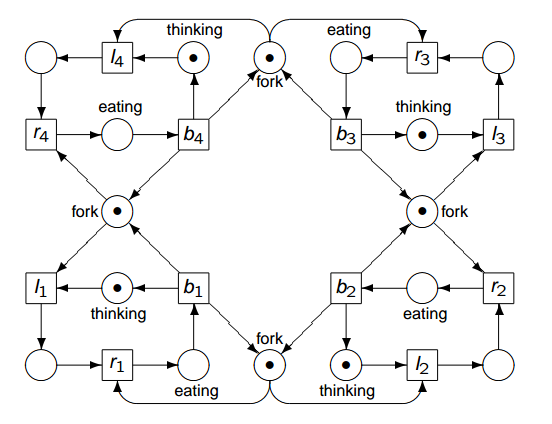
\includegraphics[scale=0.45]{graphics/dining_philosophers.png}
        \caption{Filósofos comensales \citep{Labri}}
    \end{figure}
\end{frame}

%%%%%%%%%%%%%%%%%%%%%%%%%%%%%%%%%%%%%%%%%%%%%%%%%%%%%%

\begin{frame}{Modelos}
    \begin{itemize}
        \item{Autómatas finitos}
        \item{Actividades paralelas}
        \item{Computación de flujo de datos}
        \item{Protocolos de comunicación}
        \item{Control de sincronización}
        \item{Productor-Consumidor}
        \textbf{\item{Lenguajes formales}}
        \item{Sistemas multiprocesador}
    \end{itemize}
    \begin{itemize}
        \item Concurrencia
        \item Conflictos
        \item Confusión
            \begin{itemize}
                \item Simétrica
                \item Asimétrica
            \end{itemize}
    \end{itemize}
\end{frame}

%%%%%%%%%%%%%%%%%%%%%%%%%%%%%%%%%%%%%%%%%%%%%%%%%%%%%%

\begin{frame}{Autómatas finitos}
    \begin{figure}[h]
        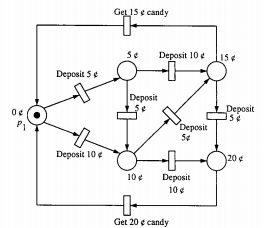
\includegraphics[scale=0.8]{graphics/af_rp.png}
        \caption{Autómata finito \citep{Murata:89}}
    \end{figure}
\end{frame}

%%%%%%%%%%%%%%%%%%%%%%%%%%%%%%%%%%%%%%%%%%%%%%%%%%%%%%

\begin{frame}{Paralelismo y concurrencia}
  \begin{columns}
    \column{.42\textwidth}
    \begin{figure}[h]
        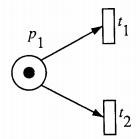
\includegraphics[scale=0.7]{graphics/concurrency_rp.png}
        \caption{Concurrencia en RP \citep{Murata:89}}
    \end{figure}
    \column{.58\textwidth}
        \begin{figure}[h]
            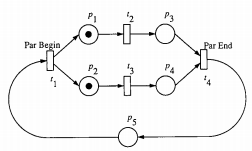
\includegraphics[scale=0.7]{graphics/parallel_activities.png}
            \caption{Sincronización en RP \citep{Murata:89}}
        \end{figure}
  \end{columns}
\end{frame}

%%%%%%%%%%%%%%%%%%%%%%%%%%%%%%%%%%%%%%%%%%%%%%%%%%%%%%

\begin{frame}{Confusión}
  \begin{columns}
    \column{.50\textwidth}
    \begin{figure}[h]
        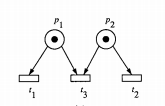
\includegraphics[scale=1]{graphics/symmetric_confusion.png}
        \caption{Confusión simétrica \citep{Murata:89}}
    \end{figure}
    \column{.50\textwidth}
        \begin{figure}[h]
            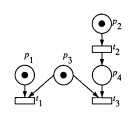
\includegraphics[scale=1]{graphics/asymmetric_confusion.png}
            \caption{Confusión asimétrica \citep{Murata:89}}
        \end{figure}
  \end{columns}
\end{frame}

%%%%%%%%%%%%%%%%%%%%%%%%%%%%%%%%%%%%%%%%%%%%%%%%%%%%%%

\begin{frame}{Métodos de análisis}
    \begin{itemize}
        \item Árbol de cobertura
        \item Matriz de incidencia
    \end{itemize}
\end{frame}

%%%%%%%%%%%%%%%%%%%%%%%%%%%%%%%%%%%%%%%%%%%%%%%%%%%%%%

\begin{frame}{Árbol de cobertura - Marcados frontera}
    \begin{itemize}
        \item Marcados muertos
        \item Nodos duplicados
        \item Marcados que sólo se diferencian del anterior por tener un número distinto de \textit{tókens} en alguna plaza y que habilita el mismo conjunto de transiciones. Se remplaza la plaza con la cantidad de tókens distinta por el símbolo $\omega$
    \end{itemize}
\end{frame}

%%%%%%%%%%%%%%%%%%%%%%%%%%%%%%%%%%%%%%%%%%%%%%%%%%%%%%

\begin{frame}{Árbol de cobertura}
    \begin{figure}[h]
        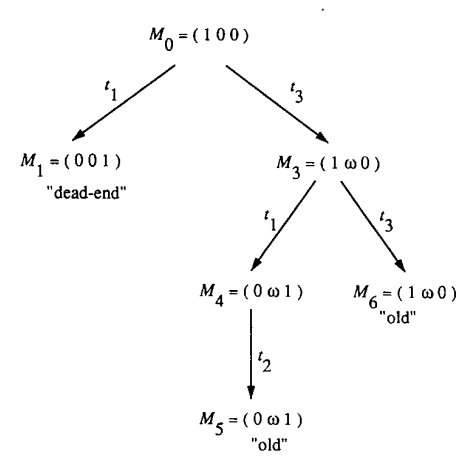
\includegraphics[scale=0.45]{graphics/reachability_tree.png}
        \caption{Árbol de cobertura \citep{Murata:89}}
    \end{figure}
\end{frame}

%%%%%%%%%%%%%%%%%%%%%%%%%%%%%%%%%%%%%%%%%%%%%%%%%%%%%%

\begin{frame}{Matriz de incidencia}

    Sea una RP = (P, T, I, O) con \textit{n} plazas y \textit{m} transiciones, se define la \textbf{matriz de incidencia previa} como: 
    \begin{equation}
        C^-(j, i) = I(p_i, t_j)
    \end{equation}
    Se define la \textbf{matriz de incidencia posterior} como:
    \begin{equation}
        C^+(j, i) = O(t_j, p_i)
    \end{equation}
    Se define la \textbf{matriz de incidencia} como:
    \begin{equation}
        C = C^+ - C^-
    \end{equation}
\end{frame}

%%%%%%%%%%%%%%%%%%%%%%%%%%%%%%%%%%%%%%%%%%%%%%%%%%%%%%

\begin{frame}{Representación matricial}

    Una transición $t_j$ se define por un vector $e_j$ de dimensión \textit{m} de componentes:

        \[ e_j(i) =
          \begin{cases}
            1       & \text{si } i = j\\
            0       & \text{si } i \neq j
          \end{cases}
        \]
    Una transición $t_j$ está habilitada en un marcado \textit{M} si
    \begin{equation}
        M \geq e_j \bullet C^-
    \end{equation}
    El resultado del disparo de la transición $t_j$ a partir del estado \textit{M} es:
    \begin{equation}
        M' = M + e_j \bullet C
    \end{equation}

\end{frame}

%%%%%%%%%%%%%%%%%%%%%%%%%%%%%%%%%%%%%%%%%%%%%%%%%%%%%%

\begin{frame}{Propiedades de comportamiento}
    \begin{itemize}
        \item{Alcanzabilidad}
        \item{Límite}
            \begin{itemize}
                \item{Seguridad}
            \end{itemize}
        \item{Vitalidad}
        \item{Estado base}
        \item{Cobertura}
        \item{Persistencia}
        \item{Justicia}
    \end{itemize}
\end{frame}

%%%%%%%%%%%%%%%%%%%%%%%%%%%%%%%%%%%%%%%%%%%%%%%%%%%%%%

\begin{frame}{Lenguajes formales y RP}
    \begin{itemize}
        \item{Clases}
        \item{Expresividad}
    \end{itemize}
\end{frame}

%%%%%%%%%%%%%%%%%%%%%%%%%%%%%%%%%%%%%%%%%%%%%%%%%%%%%%

\begin{frame}{Definición de los lenguajes RP}
    Para que una RP pueda ser reconocedora de lenguajes, se deben definir tres conceptos más:
    \begin{itemize}
        \item{Estado inicial}
        \item{Etiquetado $ \sigma: T \mapsto \Sigma$}
        \item Estado final
    \end{itemize}
\end{frame}

%%%%%%%%%%%%%%%%%%%%%%%%%%%%%%%%%%%%%%%%%%%%%%%%%%%%%%

\begin{frame}{Conjunto de estados finales}
    Según cómo se defina el conjunto de estados finales de una RP reconocedora, el lenguaje reconocido será distinto \citep{Peterson:81}
    \begin{itemize}
        \item{Tipo-L = $\{\sigma(\beta) \in \Sigma^*, \quad \beta \in T^* \text{ y }\delta(M_0, \beta) \in F\}$}
        \item{Tipo-G = $\{\sigma(\beta) \in \Sigma^*, \quad \beta \in T^* \text{ y } \exists M_f \in F \text{ tal que } \delta(M_0, \beta) \geq M_f\}$}
        \item{Tipo-T = $\{\sigma(\beta) \in \Sigma^*, \quad \beta \in T^* \text{ y } \delta(M_0, \beta) \text{ está definido } \forall t_j \in T, \quad \delta(\delta(M_0, \beta), t_j) \text{ no está definido } \}$}
        \item{Tipo-P = $\{\sigma(\beta) \in \Sigma^*, \quad \beta \in T^* \text{ y } \delta(M_0, \beta) \text{ está definido }\}$}
    \end{itemize}

    \hfill \break 
    $\beta$ es una secuencia de transiciones.

    $\delta: M \times \beta \mapsto M$
\end{frame}


%%%%%%%%%%%%%%%%%%%%%%%%%%%%%%%%%%%%%%%%%%%%%%%%%%%%%%

\begin{frame}{Clases de lenguajes RP}
    \begin{figure}[h]
        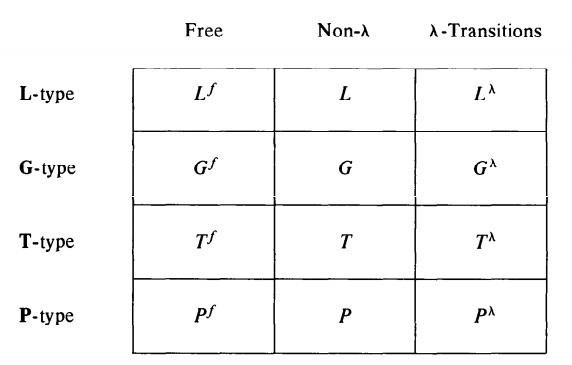
\includegraphics[scale=0.45]{graphics/rp_languages.png}
        \caption{12 clases de lenguajes reconocidos por Redes de Petri \citep{Peterson:81}}
    \end{figure}
\end{frame}

%%%%%%%%%%%%%%%%%%%%%%%%%%%%%%%%%%%%%%%%%%%%%%%%%%%%%%

\begin{frame}{Expresividad}
    \begin{figure}[h]
        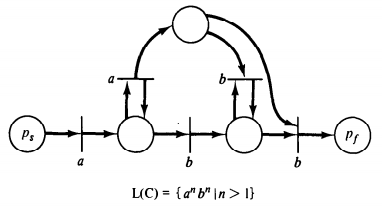
\includegraphics[scale=0.7]{graphics/rp_context_free.png}
        \caption{Red de petri reconocedora del lenguajes libre de contexto \citep{Peterson:81}}
    \end{figure}
\end{frame}

%%%%%%%%%%%%%%%%%%%%%%%%%%%%%%%%%%%%%%%%%%%%%%%%%%%%%%

\begin{frame}{Expresividad}
    \begin{figure}[h]
        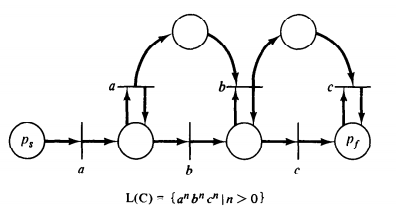
\includegraphics[scale=0.7]{graphics/rp_context_sensitive.png}
        \caption{Red de petri reconocedora del lenguajes sensibles al contexto \citep{Peterson:81}}
    \end{figure}
\end{frame}

%%%%%%%%%%%%%%%%%%%%%%%%%%%%%%%%%%%%%%%%%%%%%%%%%%%%%%

\begin{frame}{Expresividad}
    \begin{figure}[h]
        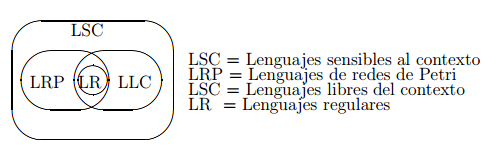
\includegraphics[scale=0.6]{graphics/rp_chomsky.png}
        \caption{Lenguajes de RP en la clasificación de Chomsky \citep{Augusto:95}}
    \end{figure}
\end{frame}

%%%%%%%%%%%%%%%%%%%%%%%%%%%%%%%%%%%%%%%%%%%%%%%%%%%%%%

%%%%%%%%%%%%%%%%%%%%%%%%%%%%%%%%%%%%%%%%%%%%%%%%%%%%%%%
%\begin{frame}
  %\frametitle{Temario}

%% TODO
  
%\end{frame}
%%%%%%%%%%%%%%%%%%%%%%%%%%%%%%%%%%%%%%%%%%%%%%%%%%%%%%%
%\begin{frame}[label=frameoptions]
\frametitle{The frame environment}

  \hspace{-1em}{\tt $\backslash$begin\{frame\}[OVERLAY OPTION][OPTIONS]\{Title\}\{Subtitle\}}

  \bigskip

  {\bf OVERLAY OPTION:}
  \begin{itemize}
  \item {\tt <+->} 
  \end{itemize}

  \bigskip

  {\bf OPTIONS:}
  \begin{itemize}
  \item {\tt b,c,t}: frame orientation
  \item {\tt squeeze}: minimizes vertical margins
  \item {\tt plain}: suppresses title, header and sidebar
  \item {\tt label=name}: makes a frame reusable with {\tt $\backslash$againframe\{name\}} and can be used with hyperlinks.
  \item {\tt allowframebreaks}: spread frame content over several slides 
  \end{itemize}

  \vfill 

  Hyperlink: \hyperlink{frameoptions}{\beamerbutton{The frame environment}}

\end{frame}
\begin{frame}
  \frametitle{Blocks}

  \begin{block}{Title of a block}		% Titles may be left blank!
    Body of a block
  \end{block}

  \begin{exampleblock}{Title of an exampleblock}
    Body of an exampleblock
  \end{exampleblock}

  \begin{alertblock}{Title of an alertblock}
    Body of an alertblock
  \end{alertblock}
  
\end{frame}

\begin{frame}
  \frametitle{Overlays}
  {\small 

    Explicit specification of overlays:
    \begin{itemize}
    \item \color<2>{red}{Changing colors ...}
    \item \alert<3>{Alert mode ...} 
    \item \textbf<4>{Changing the font face ...}
    \item \only<-5>{Changing existence ...} 
    \item \visible<-6>{Changing visability ...}
    \item \uncover<7->{Uncovering from grey ...}
    \item \alt<8>{Specifying alternations ...}{... in one instruction}
    \end{itemize}

    \vfill
    {\tt $\backslash$pause[<number>]} separates two overlays.

    \vfill
    Overlays in list environments:
    \begin{itemize}
    \item<9-> First item
    \item<alert@10> Second item with alert
    \item Alternatively, list environments can have an overlay option such as {\tt <+-> } or {\tt <+- alert@ +>}.
    \end{itemize}

    \vfill
    Remember that you can declare overlays in the frame options.
    \hyperlink{frameoptions}{\beamerbutton{The frame environment}}

  }
\end{frame}

\begin{frame}
  \frametitle{Columns}

  \begin{columns}
    \column{.55\textwidth}
    First column
		\pgfimage[width=\textwidth]{graphics/hhu-logo-hres}
    \column{.45\textwidth}
		Second column
    \begin{enumerate}
    \item bla
    \item blupp
    \end{enumerate}
  \end{columns}

\end{frame}


\begin{frame}
\frametitle{Citation}
Example for invoking citations: \cite{Bech:63}, \citet[291]{Bech:63}, \citep{Bech:63}, \citealt{Bech:63}

References are stored in \texttt{references.bib}.

\end{frame}

\begin{frame}
\frametitle{Linguistic examples}
\ex. This is a simple example.

\exg. [Noch am Boden liegend$_i$], sei [auf ihn$_i$] eingetreten worden.\\
still on.the floor lying be on him PART.kicked got\\
`While he was still on the floor he was kicked.'\\
(Cf. (422) in \citep{Mueller:02})

\noindent $\Rightarrow$ \url{http://texdoc.net/texmf-dist/doc/latex/linguex/linguex-doc.pdf} \\
Note the Leipzig glossing rules: \url{http://www.eva.mpg.de/lingua/resources/glossing-rules.php}

\end{frame}

\begin{frame}
\frametitle{Trees}
\Forest{
  [S [NP] 
  [VP [V  [\textit{eats}] ]
  [NP] ]]
}

\noindent $\Rightarrow$ \url{http://mirrors.ctan.org/graphics/pgf/contrib/forest/forest-doc.pdf}

\end{frame}

\begin{frame}
\frametitle{AVM}
\begin{avm}
  \@0\[\asort{eating}
    actor & \@1 \\ 
    theme & \@2 \]
\end{avm}

\noindent $\Rightarrow$ \url{http://nlp.stanford.edu/manning/tex/avm-doc.pdf}

\end{frame}

\begin{frame}
\frametitle{IPA symbols}
\ex. \textipa{[""Ekspl@"neIS@n]}

$\Rightarrow$ \url{http://en.wikibooks.org/wiki/LaTeX/Linguistics#IPA_characters}


\end{frame}

\begin{frame}
\frametitle{Formulae}
Formulae in texts: $a^2 + b^2 = c^2$

\noindent Formulae in equation environment:
\begin{equation}
a^2 + b^2 = c^2
\end{equation}
$\Rightarrow$ \url{http://en.wikibooks.org/wiki/LaTeX/Mathematics}

\end{frame}

\begin{frame}
\frametitle{Tables}
\begin{tabular}{c|c|c}
\hline
cell 11 & cell 12 & cell 13 \\
\hline
cell 21 & cell 22 & cell 23 \\
\hline
\end{tabular}


\end{frame}

%%%%%%%%%%%%%%%%%%%%%%%%%%%%%%%%%%%%%%%%%%%%%%%%%%%%%%% 
\begin{frame}[plain,allowframebreaks]
\frametitle{Referencias}

\insertBib

\end{frame}
%%%%%%%%%%%%%%%%%%%%%%%%%%%%%%%%%%%%%%%%%%%%%%%%%%%%%%%


\end{document}

%%% Local Variables:
%%% mode: latex
%%% TeX-master: t
%%% End:
